\section{Cálculo del histograma de una imagen.}

Se nos proporciona un código el cual implementa en CUDA C, para ejecución en la CPU o en la GPU,
el cálculo del histograma de una imagen en escala de grises. Gracias a un histograma podemos
conocer la cantidad de ocurrencias que tenemos en una imagen para un color determinado.

\section{Generalización del \textit{kernel} proporcionado.}

El código que se nos proporciona asume un tamaño de bloque de 256 hebras, el número de tonos de
gris distintos que puede tomar la imagen. Se nos pide generalizar el número de hebras con que se
invoca al \textit{kernel}. Para ello necesitaremos poder inicializar a cero el \textit{array}
independientemente del número de hebras, similar para el caso de la adición sobre el histograma
que comparten todos los bloques.

Una solución es que cada hebra haga estas operaciones sobre el
dato que le corresponda según su número de hebra y este número más cualquier múltiplo de la dimensión
de bloque, siempre y cuando este índice resultante sea mayor que cero y menor que el número de tonos
de gris distintos que puede tomar la imagen.

\begin{figure}[H]
    \centering
    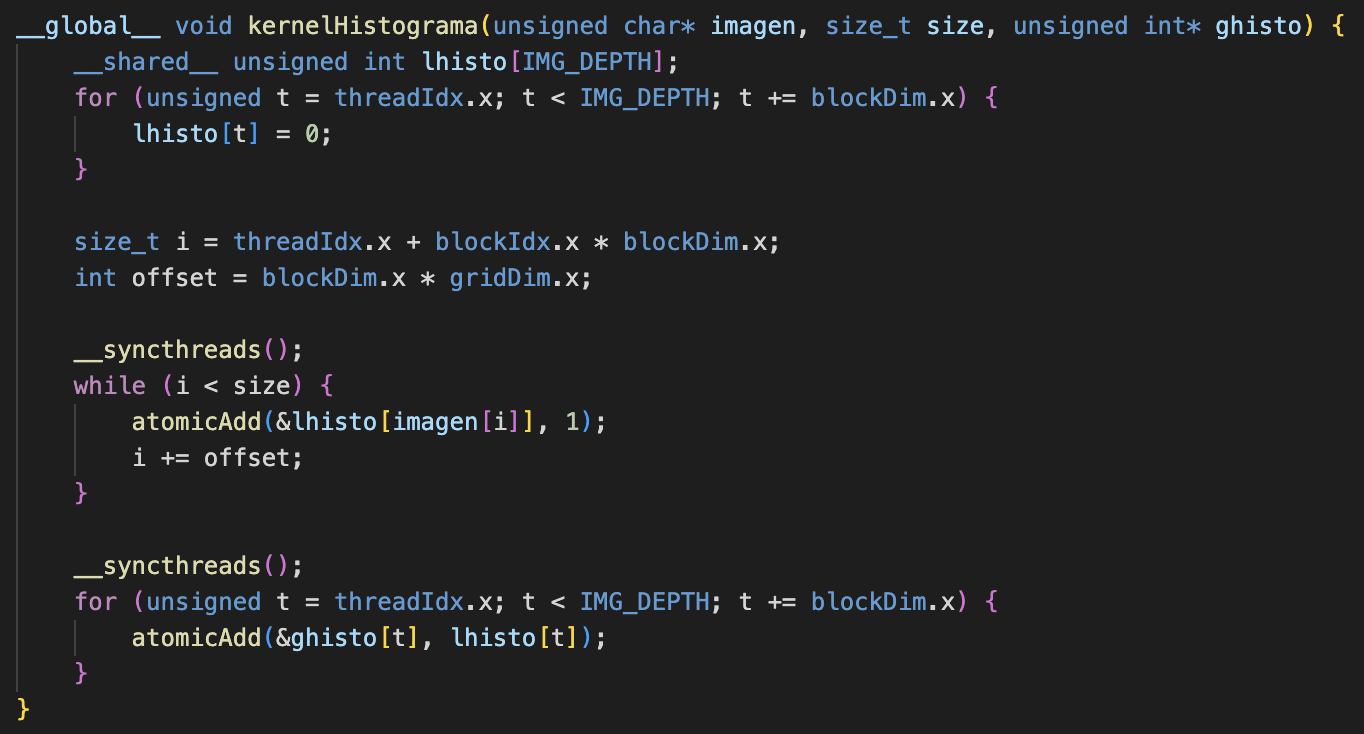
\includegraphics[width=\textwidth]{kernel.png}
    \caption{Implementación del algoritmo en \texttt{CUDA C}. El atributo \texttt{\_\_global\_\_} nos indica que es código invocable
    desde el \textit{host}. Por otra parte, \texttt{\_\_shared\_\_} nos indica que es memoria accesible por las hebras dentro de un
    mismo bloque. Por último, las funciones \texttt{\_\_syncthreads} y \texttt{atomicAdd} nos permiten imponer barreras y sumar
    en exclusión mutua un número a si mismo y almacenarlo, respectivamente.}
\end{figure}

